\documentclass[1]{report}
\usepackage[utf8]{inputenc}
\usepackage[T1]{fontenc}
\usepackage[francais]{babel}
\usepackage{listings}
\usepackage{hyperref}
\usepackage{graphicx}
\usepackage{caption}
\usepackage{xcolor}
\usepackage{sectsty}

\hypersetup{ %Paramètres pour les liens hypertextes
	colorlinks=true,
	linktoc=all,
	linkcolor=blue,
	urlcolor=blue,
}

\title{\textcolor{red}{Projet KenKen2 : Analyse des besoins}}
\author{Erwan Dupland, Sébastien Granger, Hugo Jalenques, Pablo Tomas
\\ Client : Emmanuel Fleury \\ Chargé de TD : Simon Archipoff}
\date{Rendu du 01 Février 2019}

\begin{document}

\chapterfont{\color{red}}
\sectionfont{\color{blue}}

\maketitle

\chapter{Introduction}

		Le but de ce projet est de concevoir un programme capable de résoudre et de générer des grilles pour le jeu KenKen. \\~\\

		Le Kenken est un jeu mathématique dérivé du sudoku, qui consiste à compléter une grille par des chiffres en les trouvant par déduction ou par calcul. La grille est constituée d'un nombre égal de lignes et de colonnes contenant des blocs de deux ou trois cases délimitées par un épais trait noir. Le chiffre inscrit en haut à gauche de chaque bloc est le résultat de l'opération (addition, soustraction, multiplication, division) effectuée avec
		les chiffres des deux ou trois cases d'un même bloc.\\~\\

		Comme pour le sudoku, le but du jeu est de remplir toutes les cases de la grille avec des chiffres allant de 1 à n (n étant le nombre de lignes et de
		colonnes du tableau) sans jamais avoir deux fois le même chiffre dans la même colonne ou sur la même ligne.

\chapter{Analyse des besoins}

    \begin{center}

        \textbf{Ouvrir le git sur savane à l'adresse} : \href{https://services.emi.u-bordeaux.fr/projet/savane}{git}

    \end{center}

    \section{Besoins fonctionnels}

        Le logiciel demandé devra avoir deux modes : \\

        \begin{itemize}

            \item \textbf{Résolution de grilles} : \\

        \quad Différents algorithmes de résolution de grilles seront à implémenter et pourront être choisis par l'utilisateur. Par exemple, nous pouvons mettre à disposition un algorithme dit de logique et un algotithme de Backtracking.
        \\

     \quad L'utilisateur peut alors choisir avec une option adaptée quel algorithme sera appelé pour résoudre la grille. Il aura aussi la possibilité de comparer les différents algorithmes qu'il utilisera sur une même grille pour savoir lequel sera le plus rapide.
\\

		\quad	Des statistiques pertinentes seront donc affichées après la résolution des grilles pour permettre à l'utilisateur d'effectuer cette comparaison.	Une option \emph{-a}, \emph{--all} cherchera \textbf{toutes} les solutions possibles, \textbf{priorité : essentiel}.
\\

        \quad    Des tests de contrôle seront appelés avec un jeu de grilles de référence dont les solutions sont connues. Nos algorithmes retourneront exactement les mêmes solutions pour passer ces tests.
\\

        \quad    Une option \emph{-FILE}, \emph{--output FILE} permettra d'écrire les résultats dans un fichier, \textbf{priorité : essentiel}. Des tests permettront de vérifier que les fichiers satisferont l'entrée attendue, au bon format.



            \item \textbf{Génération de grilles (N*N)} : \\

            Par défaut, la taille d'une grille est 6*6.

            Le format d'entrée d'une grille à générer sera le suivant : \\

            %\fbox{\parbox{3cm}{
            % \# Rooms \\
            % 1  2  2  3  4  4 \\
            % 1  5  5  3  6  4 \\
            % 7  7  8  8  6  4 \\
            % 7  7  9 10 11 11 \\
            %12 12  9 10 10 13 \\
            %14 14 14 15 15 13 \\
            %}}
            \begin{center}

                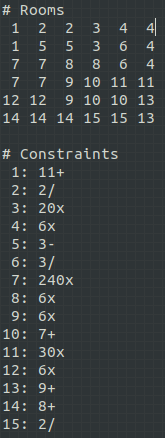
\includegraphics[width=4cm]{Entree.png}

            \end{center}

            Les caractères reconnus seront donc : '\emph{\#}', '\emph{0-9}', '\emph{:}', '\emph{+}', '\emph{-}', '\emph{x}', '\emph{/}', \textbf{priorité : essentiel}.

            Tout autre caractère (en dehors d'un commentaire) devra provoquer une erreur.

            Ici, des tests de validité se feront en passant des caractères "interdits", nous permettant de constater qu'une erreur est bien induite.

            Le format de sortie des grilles résolues sera le suivant : \\

            \begin{center}

                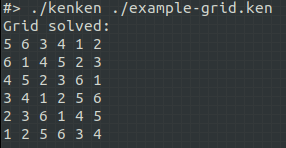
\includegraphics[width=4cm]{Sortie.png}

            \end{center}



            Des options \emph{-V}, \emph{--version} et \emph{-h}, \emph{--help} permettront de connaître la version du logiciel en cours et d'afficher une aide à l'utilisateur en affichant notamment toutes les options disponibles (citées précedemment), \textbf{priorité : essentiel}. \\

            Une option \emph{-u}, \emph{--unique} permettra de générer une grille avec une \textbf{unique} solution, \textbf{priorité : conditionnel}. \\

            Nous pouvons, de plus, nous engager à créer toutes les grilles de taille 3*3. En effet, le nombre de grilles 3*3 reste relativement raisonnable, le fait de toutes les générer est donc un bon moyen de tester notre implémentation. \\




			\item \textbf{Corpus de grilles, priorité : conditionnel} : \\

		\quad	Un corpus de grilles sera fourni, contenant des instances difficiles résolubles en un temps long.

			Un des buts du projet étant aussi de savoir jusqu'où nos algorithmes seront efficaces, ce corpus de grilles testera les limites de notre implémentation. \\



			\item \textbf{Parallélisme, priorité : conditionnel} : \\

		\quad	Il est demandé de paralléliser le code pour bénéficier d'architectures multicoeurs, cette étape sera réalisée en utilisant OpenMP.
\\


        \end{itemize}

        Le logiciel s'interrompra en renvoyant un code \emph{EXIT\_FAILURE} en cas d'erreur ou renverra code \emph{EXIT\_SUCCESS} si tout s'est déroulé normalement.

        Le logiciel sera programmé en C11.

        Des grilles de tests avec une couverture de code d'au moins 90\% seront fournies. \\

    \section{Besoins non-fonctionnels}

        Efficacité/rapidité du logiciel : une analyse d'efficacité en profondeur sera menée sur les différentes approches tentées, \textbf{priorité : essentiel}.

		Il est important de garder à l'esprit qu'une tentative d'approche très efficace sur une grille précise, le sera peut-être moins sur une autre grille présentant des conditions différentes.

        Du profiling sera donc effectué pour tester les différentes performances de nos algorithmes, \textbf{priorité : essentiel}.

        Les algorithmes (utilisant le backtracking) qui existent déjà permettent de résoudre des grilles 4*4 en un temps très court : de l'ordre de 60ms. En ce qui concerne les grilles 5*5, la temps de résolution est de 100ms en moyenne. On passe à 170ms pour les grilles 6*6, 800ms pour les grilles 7*7 et on observe une grande augmentation de cette durée en ce qui concerne les grilles 8*8 : de 1,5 min à 20 min. \\

        A propos de la génération, nous pouvons laisser à l'utilisateur le choix de construire des grilles possédant des niveaux de difficultés différents, \textbf{priorité : conditionnel}. \\




        Une option \emph{-v}, \emph{--verbose}, commune à la résolution et à la génération, permettra de choisir l'algorithme à utiliser et devra renseigner l'utilisateur sur les différentes étapes internes de la résolution ou de la génération des grilles et donner quelques statistiques, \textbf{priorité : essentiel}. \\





\chapter{Diagramme de Gantt}


     \begin{center}

                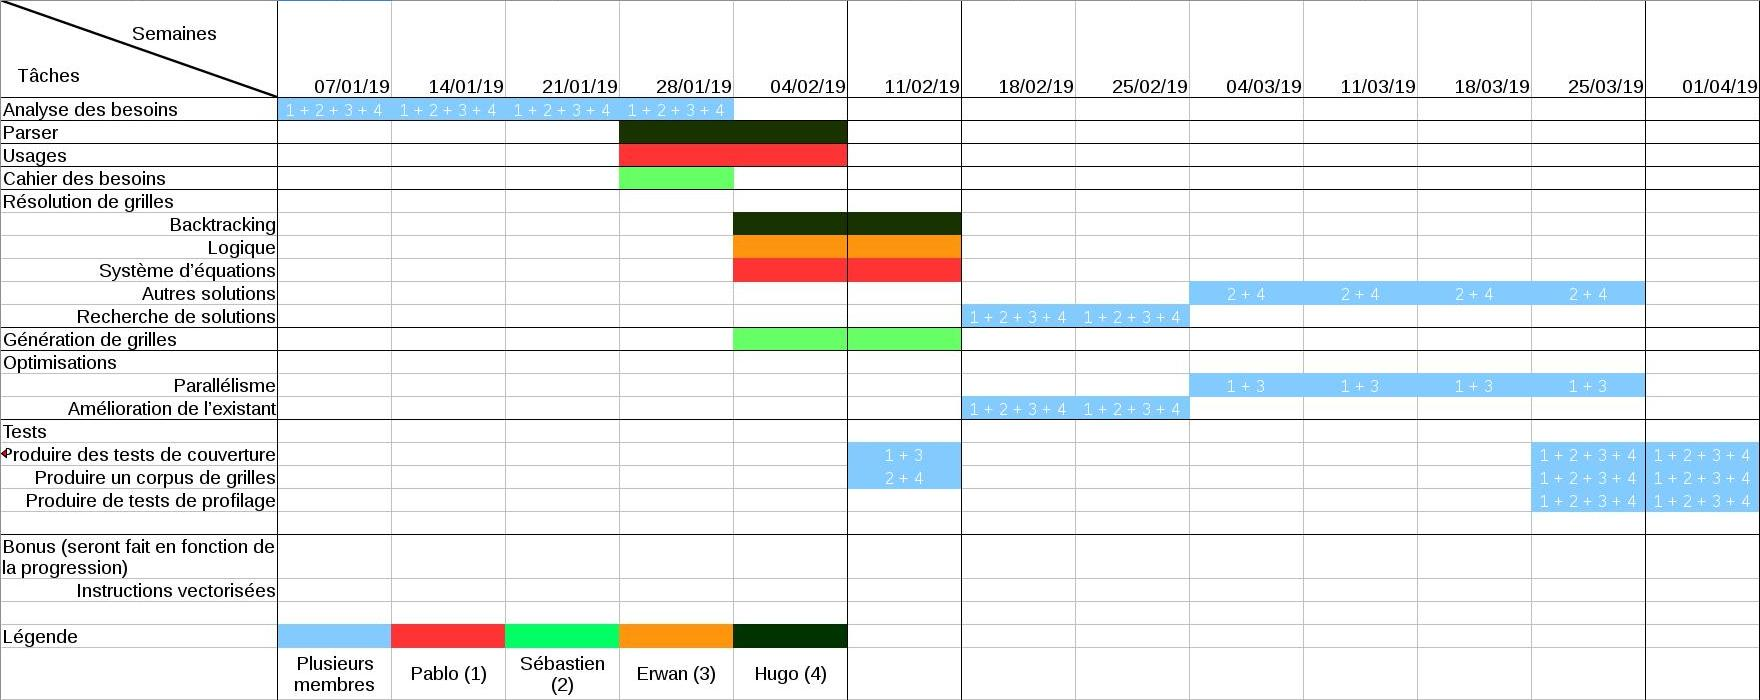
\includegraphics[width = 15cm]{Gantt.jpg}

    \end{center}

    \quad Ci-dessus le diagramme de Gantt représentant l'organisation de notre projet pour les semaines à venir. Il est à retrouver en meilleure qualité sur le git (doc/Gantt.jpg).


\chapter{Scénario}

		En premier lieu, l'utilisateur pourra afficher toutes les options disponibles grâce à l'option \emph{-h}.

		Ensuite, s'il veut s'informer de la version du logiciel, l'option \emph{-V} la lui indiquera.

		Admettons que l'utilisateur veuille générer une grille et la résoudre.

		Il devra exécuter les deux commandes suivantes :

\\~\\

	./kenken -g[N] -o FILE1 (N étant la taille de la grille).



	./kenken -o FILE2 -V FILE1


\chapter{Bibliographie}

    $\rightarrow$ Articles \\

    \begin{itemize}

        \item Labri

        		\emph{Titre} : KenKen Puzzle Solver using Backtracking Algorithm

        		\emph{Auteur} : Asanilta Fahda

        		\emph{URL} : \href{http://www.labri.fr/perso/fleury/courses/pdp/Puzzle_Games/KenKen/KenKen_Puzzle_Solver_using_Backtracking_Algorithm.pdf}{KenKen Puzzle Solver using Backtracking Algorithm}{Using Backtracking Algorithm}



        		\emph{Date} : 05/05/2015 \\

		\item Labri

				\emph{Titre} : An Efficient Algorithm for Constructing all Magic Squares of Order Four

				\emph{Auteur} : Changyu Liu, Tiezhu Zhao et Bin Lu

				\emph{URL} : \href{http://www.labri.fr/perso/fleury/courses/pdp/Puzzle_Games/KenKen/23.pdf}{Constructing all Magic Squares of Order Four}



				\emph{Date} : 2015 \\

		\item Labri

				\emph{Titre} : How Simple Algorithms Can Solve Latin Square Completion-Type Puzzles Approximately

				\emph{Auteur} : Kazuya Haraguchi et Hirotaka Ono

				\emph{URL} : \href{http://www.labri.fr/perso/fleury/courses/pdp/Puzzle_Games/KenKen/23_276.pdf}{Solve Latin Square}



				\emph{Date} : 05/2015 \\

    \end{itemize}

    $\rightarrow$ Sites internet \\

    \begin{itemize}

		\item Community Wolfram

			\emph{Titre} : Solving a KenKen puzzle using logic

			\emph{Auteur} : Sander Huisman

			\emph{URL} : \href{https://community.wolfram.com/groups/-/m/t/613040}{Solving a KenKen Puzzle Using Logic}

			\emph{Date} : Dernière édition : 12/12/2018 \\


        \item Mlsite

            \emph{Titre} : Inconnu

            \emph{Auteur} : Inconnu

            \emph{URL} : \href{http://www.mlsite.net/neknek/?fbclid=IwAR2uaILVfEVoqUzZFhEE7PmyQz7L9yb4JMFeXe8C8y4nL40hgjXXnMf4JCg}{Mlsite}

            \emph{Date} : Inconnue

    \end{itemize}


\end{document}
